\documentclass{article}
\usepackage{physics}
\usepackage{graphicx}
\usepackage{caption}
\usepackage{amsmath}
\usepackage{bm}
\usepackage{framed}
\usepackage{authblk}
\usepackage{empheq}
\usepackage{amsfonts}
\usepackage{esint}
\usepackage[makeroom]{cancel}
\usepackage{dsfont}
\usepackage{centernot}
\usepackage{mathtools}
\usepackage{bigints}
\usepackage{amsthm}
\theoremstyle{definition}
\newtheorem{defn}{Definition}[section]
\newtheorem{prop}{Proposition}[section]
\newtheorem{rmk}{Remark}[section]
\newtheorem{thm}{Theorem}[section]
\newtheorem{exmp}{Example}[section]
\newtheorem{prob}{Problem}[section]
\newtheorem{sln}{Solution}[section]
\newtheorem*{prob*}{Problem}
\newtheorem{exer}{Exercise}[section]
\newtheorem*{exer*}{Exercise}
\newtheorem*{sln*}{Solution}
\usepackage{empheq}
\usepackage{tensor}
\usepackage{xcolor}
%\definecolor{colby}{rgb}{0.0, 0.0, 0.5}
\definecolor{MIT}{RGB}{163, 31, 52}
\usepackage[pdftex]{hyperref}
%\hypersetup{colorlinks,urlcolor=colby}
\hypersetup{colorlinks,linkcolor={MIT},citecolor={MIT},urlcolor={MIT}}  
\usepackage[left=1in,right=1in,top=1in,bottom=1in]{geometry}

\usepackage{newpxtext,newpxmath}
\newcommand*\widefbox[1]{\fbox{\hspace{2em}#1\hspace{2em}}}

\newcommand{\p}{\partial}
\newcommand{\R}{\mathbb{R}}
\newcommand{\C}{\mathbb{C}}
\newcommand{\lag}{\mathcal{L}}
\newcommand{\nn}{\nonumber}
\newcommand{\ham}{\mathcal{H}}
\newcommand{\M}{\mathcal{M}}
\newcommand{\I}{\mathcal{I}}
\newcommand{\K}{\mathcal{K}}
\newcommand{\F}{\mathcal{F}}
\newcommand{\w}{\omega}
\newcommand{\lam}{\lambda}
\newcommand{\al}{\alpha}
\newcommand{\be}{\beta}
\newcommand{\x}{\xi}

\newcommand{\G}{\mathcal{G}}

\newcommand{\f}[2]{\frac{#1}{#2}}

\newcommand{\ift}{\infty}

\newcommand{\lp}{\left(}
\newcommand{\rp}{\right)}

\newcommand{\lb}{\left[}
\newcommand{\rb}{\right]}

\newcommand{\lc}{\left\{}
\newcommand{\rc}{\right\}}


\newcommand{\V}{\mathbf{V}}
\newcommand{\U}{\mathcal{U}}
\newcommand{\Id}{\mathcal{I}}
\newcommand{\D}{\mathcal{D}}
\newcommand{\Z}{\mathcal{Z}}

%\setcounter{chapter}{-1}


\usepackage{enumitem}



\usepackage{subfig}
\usepackage{listings}
\captionsetup[lstlisting]{margin=0cm,format=hang,font=small,format=plain,labelfont={bf,up},textfont={it}}
\renewcommand*{\lstlistingname}{Code \textcolor{violet}{\textsl{Mathematica}}}
\definecolor{gris245}{RGB}{245,245,245}
\definecolor{olive}{RGB}{50,140,50}
\definecolor{brun}{RGB}{175,100,80}

%\hypersetup{colorlinks,urlcolor=colby}
\lstset{
	tabsize=4,
	frame=single,
	language=mathematica,
	basicstyle=\scriptsize\ttfamily,
	keywordstyle=\color{black},
	backgroundcolor=\color{gris245},
	commentstyle=\color{gray},
	showstringspaces=false,
	emph={
		r1,
		r2,
		epsilon,epsilon_,
		Newton,Newton_
	},emphstyle={\color{olive}},
	emph={[2]
		L,
		CouleurCourbe,
		PotentielEffectif,
		IdCourbe,
		Courbe
	},emphstyle={[2]\color{blue}},
	emph={[3]r,r_,n,n_},emphstyle={[3]\color{magenta}}
}






\begin{document}
\begin{framed}
	\noindent Name: \textbf{Huan Q. Bui}\\
	Course: \textbf{8.309 - Classical Mechanics III}\\
	Problem set: \textbf{\#2}
\end{framed}
	
	
\noindent \textbf{1. Spherical Pendulum with Friction}
\begin{enumerate}[label = (\alph*)]
	\item In this problem, we will ignore the effect of buoyancy and assume that the effective mass $m'$ is equal to $m$, the real mass of the pendulum blob. Stokes law states that $\vec{F}_\text{friction} = -6\pi \eta R\vec{v} \equiv -b\vec{v}$, where $b>0$ is a constant which depends on the radius $R$ of the mass and the viscosity $\mu$ of the fluid. Putting this force in the form $F_i = -h_i(v_i) \vec{v}_i/v_i$, we find that $h_i = b v_i$. Thus, the dissipation function is 
	\begin{equation*}
	\mathcal{F} = \sum_{i=1}^3  \int_0^{v_i}h_i(v_i') \,dv_i' = \f{1}{2}b(\dot{x}^2+\dot{y}^2+\dot{z}^2).
	\end{equation*}
	We choose the spherical coordinates such that the origin is the pivot of the pendulum and $\theta = \pi$ when the pendulum is in its equilibrium position: $(x,y,z) = (r\sin\theta\cos\phi, r\sin\theta\sin\phi,r\cos\theta)$, we find 
	\begin{equation*}
	\mathcal{F} = \f{1}{2}b\lb \dot{r}^2 + r^2(\dot{\theta}^2 + \sin^2\theta \dot{\phi}^2) \rb = 
	\f{b}{2}\lb \dot{r}^2 + r^2(\dot{\theta}^2 + \sin^2\theta \dot{\phi}^2) \rb = 
	\boxed{\f{bl^2}{2}(\dot{\theta}^2 + \sin^2\theta \dot{\phi}^2)}
	\end{equation*}
	where we have used $r=l$ which is fixed. 
	
	\item The Lagrangian is 
	\begin{align*}
	\lag &= T-U\\
	&=  \f{1}{2}m\dot{\vec{r}}^2 - mgr\cos\theta\\
	&= \f{m}{2}\lb \dot{r}^2 + r^2(\dot{\theta}^2+\sin^2\theta\dot{\phi}^2) \rb - mgr\cos\theta \\
	&= \f{ml^2}{2}\lp \dot{\theta}^2 + \sin^2\theta \dot{\phi}^2 \rp - mgl\cos\theta
	\end{align*}
	where we have used $r=l$ which is fixed. We find two equations of motion:
	\begin{align*}
	\f{d}{dt}\lp \f{\p \lag}{\p \dot{\theta}} \rp - \f{\p \lag}{\p \theta} = \f{-\p \mathcal{F}}{\p \dot{\theta}} 
	&\implies l^2 m \ddot{\theta} - glm \sin\theta + l^2 m \cos\theta\sin\theta \dot{\phi}^2 = -bl^2 \dot{\theta}\\
	&\implies  \boxed{\ddot{\theta}  = -\f{b\dot{\theta}}{m}+\f{ \sin\theta }{l} \lb  g + l\cos\theta \dot{\phi}^2 \rb}
	\end{align*}
	and 
	\begin{align*}
	\f{d}{dt}\lp \f{\p \lag}{\p \dot{\phi}} \rp - \f{\p \lag}{\p \phi} = \f{-\p \mathcal{F}}{\p \dot{\phi}} 
	&\implies l^2 m \sin\theta \left(2 \dot\theta \cos\theta \dot\phi+\sin\theta \ddot{\phi}\right) = -bl^2 \sin^2\theta \dot{\phi} \\
	&\implies \boxed{\ddot{\phi} = -\f{\dot{\phi}( b + 2m \cot \theta \dot{\theta})}{m}}
	\end{align*}
	
	
	\item Mathematica code:
	\begin{lstlisting}
	(*Problem 1*)
	
	In[1]:= L = (m*l^2/2)*(\[Theta]'[t]^2 + Sin[\[Theta][t]]^2*\[Phi]'[t]^2) - 
	m*g*l*Cos[\[Theta][t]]
	
	Out[1]= -g l m Cos[\[Theta][t]] + 
	1/2 l^2 m (Derivative[1][\[Theta]][t]^2 + 
	Sin[\[Theta][t]]^2 Derivative[1][\[Phi]][t]^2)
	
	In[2]:= F = (b*l^2/2)*(\[Theta]'[t]^2 + Sin[\[Theta][t]]^2*\[Phi]'[t]^2)
	
	Out[2]= 1/2 b l^2 (Derivative[1][\[Theta]][t]^2 + 
	Sin[\[Theta][t]]^2 Derivative[1][\[Phi]][t]^2)
	
	In[13]:= (*Theta equation*)
	
	In[12]:= Solve[FullSimplify[
	D[D[L, \[Theta]'[t]], t] - 
	D[L, \[Theta][t]] == -D[F, \[Theta]'[t]]], \[Theta]''[
	t]] // FullSimplify
	
	Out[12]= {{(\[Theta]^\[Prime]\[Prime])[
	t] -> -((b Derivative[1][\[Theta]][t])/m) + (
	Sin[\[Theta][t]] (g + 
	l Cos[\[Theta][t]] Derivative[1][\[Phi]][t]^2))/l}}
	
	In[5]:= D[D[L, \[Theta]'[t]], t]
	
	Out[5]= l^2 m (\[Theta]^\[Prime]\[Prime])[t]
	
	In[8]:= D[L, \[Theta][t]]
	
	Out[8]= g l m Sin[\[Theta][t]] + 
	l^2 m Cos[\[Theta][t]] Sin[\[Theta][t]] Derivative[1][\[Phi]][t]^2
	
	In[9]:= -D[F, \[Theta]'[t]]
	
	Out[9]= -b l^2 Derivative[1][\[Theta]][t]
	(*Phi equation*)
	
	In[20]:= Solve[FullSimplify[
	D[D[L, \[Phi]'[t]], t] - 
	D[L, \[Phi][t]] == -D[F, \[Phi]'[t]]], \[Phi]''[
	t]] // FullSimplify
	
	Out[20]= {{(\[Phi]^\[Prime]\[Prime])[
	t] -> -(((b + 
	2 m Cot[\[Theta][t]] Derivative[1][\[Theta]][t]) Derivative[
	1][\[Phi]][t])/m)}}
	
	In[19]:= D[D[L, \[Phi]'[t]], t] // FullSimplify // TeXForm
	
	Out[19]//TeXForm=
	l^2 m \sin (\theta (t)) \left(2 \theta '(t) \cos (\theta (t)) \phi '(t)+\sin (\theta
	(t)) \phi ''(t)\right)
	
	In[16]:= D[L, \[Phi][t]]
	
	Out[16]= 0
	
	In[17]:= -D[F, \[Phi]'[t]]
	
	Out[17]= -b l^2 Sin[\[Theta][t]]^2 Derivative[1][\[Phi]][t]
	\end{lstlisting}
\end{enumerate} 


	
\noindent \textbf{2. Bead Spiraling on a Helix}
\begin{enumerate}[label = (\alph*)]
	\item The Lagrangian only has the kinetic term. In cylindrical coordinates, we have  $(x,y,z) = (r\cos\theta,r\sin\theta,z) = (bz\cos(az), bz \sin(az), z )$
	\begin{align*}
	\lag &= \f{m}{2}(\dot{x}^2 + \dot{y}^2 + \dot{z}^2)\\
	&= \f{m}{2}( \dot{r}^2 + r^2\dot{\theta}^2 +  \dot{z}^2)\\
	&= \f{m}{2}(b^2 \dot{z}^2 + a^2b^2 z^2 \dot{z}^2 + \dot{z}^2)\\
	&= \f{m}{2}(1+b^2+a^2b^2 z^2)\dot{z}^2.
	\end{align*}
	From the Euler-Lagrange equation for $z$ we find 
	\begin{align*}
	\f{d}{dt}\lp \f{\p \lag}{\p \dot{z}} \rp = \f{\p \lag}{\p z} 
	&\implies  m\ddot{z}(1+b^2 + a^2b^2 z^2) + 2ma^2b^2 z\dot{z}^2 = ma^2b^2z\dot{z}^2\\
	&\implies {\ddot{z} = \f{-a^2b^2 z\dot{z}^2}{1+b^2+a^2b^2 z^2}}
	\end{align*}
	Following the hint, we divide both sides by $\dot{z}$ and integrate:
	\begin{align*}
	\int_{0}^t \f{\ddot{z}}{\dot{z}}\,dt' = \int_{z(0)}^{z(t)}	\f{-a^2b^2 z}{1+b^2+a^2b^2 z^2}\,dz
	\implies  \ln \lp \f{\dot{z}(t)}{v_0} \rp = \ln \f{\sqrt{1+b^2+a^2b^2 h^2}}{\sqrt{1+b^2+a^2b^2 z^2}}.
	\end{align*}
	Thus, we find $\dot{z}$ as a function of $a,b,m,z,v_0,h$:
	\begin{align*}
	\boxed{\dot{z} = v_0 \sqrt{\f{1+b^2+a^2b^2h^2}{1+b^2+a^2b^2z^2}}}
	\end{align*}
	There are two ways to find the constraint torque $Z_\theta$. In the first way, we simply compute the term $(d/dt)(\p \lag/\p \dot{\theta})$ and plug in what we know about $z,\dot{z},\ddot{z}$:
	\begin{align*}
	Z_\theta &= \f{d}{dt} \lp \f{\p \lag}{\p \dot{\theta}} \rp =  \f{d}{dt}\lp mr^2\dot\theta \rp  = mb^2 a \f{d}{dt}\lp z^2\dot{z} \rp \\
	&= \boxed{mab^2 v_0^2 (1+b^2+a^2b^2h^2) \f{z(2+2b^2 +a^2b^2 z^2)}{(1+b^2 + a^2b^2 z^2)^2}}
	\end{align*}
	Alternatively, we can first find $L_z$, the $z$-component of the angular momentum, then find its rate of change to get the desired torque $Z_\theta = dL_z/dt$. The angular momentum vector is $\vec{L} = (L_x,L_y,L_z) = \vec{r}\times m\vec{v} = m(x,y,z)\times (\dot x,\dot y, \dot z)$. Using Mathematica, we find that 
	\begin{align*}
	L_z = mab^2 v_0 z^2 \sqrt{\f{1+b^2+a^2b^2h^2}{1+b^2+a^2b^2z^2}}.
	\end{align*}
	Since $\ddot{z}$ and $\dot{z}$ can ultimately be expressed in terms of $z$, we can find the desired constraint torque:
	\begin{align*}
	Z_\theta &= \f{d}{dt}L_z \\
	&= \frac{m a b^2 v_0 z\dot{z} \left(a^2 b^2 z^2+2 b^2+2\right) }{b^2 \left(a^2 h^2+1\right)+1} \left(\frac{a^2 b^2 h^2+b^2+1}{a^2 b^2 z^2+b^2+1}\right)^{3/2}\\
	&= \boxed{mab^2 v_0^2 (1+b^2+a^2b^2h^2)\f{z(2+2b^2 +a^2b^2 z^2)}{(1+b^2 + a^2b^2 z^2)^2}}
	\end{align*}
	
	
	\item The particle only has kinetic energy:
	\begin{equation*}
	E = \f{m}{2}(1+b^2+a^2b^2 z^2)\dot{z}^2.
	\end{equation*} 
	Rearranging the relation between $\dot{z}$ and $z$ gives
	\begin{align*}
	(1+b^2+a^2b^2z^2)\dot{z}^2 = (1+b^2+a^2b^2h^2)v_0^2 = \text{constant}.
	\end{align*}
	Therefore, 
	\begin{align*}
	{E = \f{m}{2}(1+b^2+a^2b^2h^2)v_0^2}
	\end{align*}
	which is constant. \\
	
	
	On the other hand, the rate of change of $L_z$ in $z$ is 
	\begin{align*}
	\f{d}{dz}L_z \propto \f{d}{dz} \lp  \f{z^2}{ \sqrt{{C+z^2}}} \rp = \f{z^3+2Cz}{(C+z^2)^{3/2}}, \quad C\text{ is a positive constant}.
	\end{align*}
	When $\abs{z}$ increases, it is clear that $L_z$ increases, as desired.  
	
	
	
	\item Mathematica code:
	\begin{lstlisting}
	In[1]:= (*Problem 2*)
	
	In[2]:= (*Lagrangian*)
	
	In[3]:= L = (m/2)*(D[x[t], t]^2 + D[y[t], t]^2 + D[z[t], t]^2)
	
	Out[3]= 1/2 m (Derivative[1][x][t]^2 + Derivative[1][y][t]^2 + 
	Derivative[1][z][t]^2)
	
	In[4]:= cyl = {x[t] -> b*z[t]*Cos[a*z[t]], 
	y[t] -> b*z[t]*Sin[a*z[t]] , z[t] -> z[t],
	D[x[t], t] -> D[b*z[t]*Cos[a*z[t]], t], 
	D[y[t], t] -> D[b*z[t]*Sin[a*z[t]], t] };
	
	In[5]:= L = L /. cyl // FullSimplify
	
	Out[5]= 1/2 m (1 + b^2 + a^2 b^2 z[t]^2) Derivative[1][z][t]^2
	
	(*Euler-Lagrange Equation for z*)
	
	In[6]:= FullSimplify[D[D[L, z'[t]], t] == D[L, z[t]]]
	
	Out[6]= a^2 b^2 m z[t] Derivative[1][z][t]^2 + 
	m (1 + b^2 + a^2 b^2 z[t]^2) (z^\[Prime]\[Prime])[t] == 0
	
	In[7]:= Solve[FullSimplify[D[D[L, z'[t]], t] == D[L, z[t]]], z''[t]]
	
	Out[7]= {{(z^\[Prime]\[Prime])[t] -> -((
	a^2 b^2 z[t] Derivative[1][z][t]^2)/(1 + b^2 + a^2 b^2 z[t]^2))}}
	
	In[8]:= Integrate[-((a^2 b^2 z[t])/(1 + b^2 + a^2 b^2 z[t]^2)), z[t]]
	
	Out[8]= -(1/2) Log[1 + b^2 + a^2 b^2 z[t]^2]
	
	In[9]:= zPrime[t] = 
	v0*Sqrt[(1 + b^2 + a^2*b^2*h^2)/(1 + b^2 + a^2*b^2*z[t]^2)]
	
	Out[9]= v0 Sqrt[(1 + b^2 + a^2 b^2 h^2)/(1 + b^2 + a^2 b^2 z[t]^2)]
	
	In[10]:= (*Torque in two ways*)
	
	In[41]:= q = 
	m*b^2*a*D[z[t]^2*z'[t], 
	t] /. {z''[t] -> -((a^2 b^2 z[t] Derivative[1][z][t]^2)/(
	1 + b^2 + a^2 b^2 z[t]^2)), 
	z'[t] -> 
	v0 Sqrt[(1 + b^2 + a^2 b^2 h^2)/(1 + b^2 + a^2 b^2 z[t]^2)]} // 
	FullSimplify
	
	Out[41]= (a b^2 m (2 (1 + b^2 (1 + a^2 h^2)) v0^2 z[t] - 
	a^2 b^2 z[t]^3 Derivative[1][z][t]^2))/(1 + b^2 + a^2 b^2 z[t]^2)
	
	In[45]:= q /. {z'[t] -> 
	v0 Sqrt[(1 + b^2 + a^2 b^2 h^2)/(
	1 + b^2 + a^2 b^2 z[t]^2)]} // Simplify
	
	Out[45]= (a b^2 (1 + b^2 (1 + a^2 h^2)) m v0^2 z[
	t] (2 + 2 b^2 + a^2 b^2 z[t]^2))/(1 + b^2 + a^2 b^2 z[t]^2)^2
	
	In[42]:= AngMom = 
	FullSimplify[
	m*Cross[{x[t], y[t], z[t]}, {D[x[t], t], D[y[t], t], 
	D[z[t], t] }] /. cyl /. {z'[t] -> zPrime[t]}]
	
	Out[42]= {-a b m v0 Cos[a z[t]] z[t]^2 Sqrt[(1 + b^2 + a^2 b^2 h^2)/(
	1 + b^2 + a^2 b^2 z[t]^2)], -a b m v0 Sin[a z[t]] z[t]^2 Sqrt[(
	1 + b^2 + a^2 b^2 h^2)/(1 + b^2 + a^2 b^2 z[t]^2)], 
	a b^2 m v0 z[t]^2 Sqrt[(1 + b^2 + a^2 b^2 h^2)/(
	1 + b^2 + a^2 b^2 z[t]^2)]}
	
	In[49]:= DAngMomZ = D[AngMom[[3]], t] // FullSimplify
	
	Out[49]= (a b^2 m v0 z[t] ((1 + b^2 + a^2 b^2 h^2)/(
	1 + b^2 + a^2 b^2 z[t]^2))^(
	3/2) (2 + 2 b^2 + a^2 b^2 z[t]^2) Derivative[1][z][t])/(1 + 
	b^2 (1 + a^2 h^2))
	
	In[51]:= DAngMomZ /. {z'[t] -> 
	v0 Sqrt[(1 + b^2 + a^2 b^2 h^2)/(
	1 + b^2 + a^2 b^2 z[t]^2)]} // FullSimplify
	
	Out[51]= (a b^2 (1 + b^2 (1 + a^2 h^2)) m v0^2 z[
	t] (2 + 2 b^2 + a^2 b^2 z[t]^2))/(1 + b^2 + a^2 b^2 z[t]^2)^2
	
	In[53]:= D[z^2/Sqrt[C + z^2], z] // FullSimplify
	
	Out[53]= (2 C z + z^3)/(C + z^2)^(3/2)
	\end{lstlisting}
\end{enumerate} 

 



\noindent \textbf{3. Hoop Rolling on a Cylinder}\\


\noindent We will assume that the hoop falls to the right. The coordinates for this problem are $(\rho,\al,\be)$ where $\rho = r+R$, $\al$ is the angle which $\vec{\rho}$ makes with the horizontal direction (measured counterclockwise from the horizontal), and $\be$ is the angle $\vec{r}$ makes with the vertical, measured clockwise from the vertical.\\

The Lagrangian is 
\begin{align*}
\lag &= T_\text{trans} + T_\text{rot} - U\\
&= \f{m}{2}\lp \dot{\rho}^2 + \rho^2 \dot{\al}^2 \rp + \f{1}{2}mr^2 \dot\beta^2 - mg\rho \sin\al.
\end{align*}
The constraint equations are
\begin{align*}
f = \rho - (r+R) = 0 \quad\quad \text{and} \quad\quad g = \dot\beta - \f{(r+R)}{r}\dot{\al} = 0.
\end{align*}
The first equation comes from the fact that the hoop is always in contact with the larger cylidner before leaving it. The second equation is due to the no-slip condition: the distance that the center of the hoop travels is the same as the distance travelled by any point on its body. We notice that $f$ is a holonomic constraint, while $g$ is semi-holonomic.\\


Let $\lambda_1, \lambda_2$ be Lagrange multipliers associated with our two constraints. The method of Lagrange multiplier states that
\begin{align*}
&\f{d}{dt}\lp \f{\p \lag}{\p \dot{\rho}} \rp - \f{\p \lag}{\p \rho} = \lambda_1 \f{\p f}{\p \rho} + \lambda_2 \f{\p g}{\p \dot{\rho}} 
\implies m\ddot{\rho} - m\rho \dot\alpha^2+mg\sin\al = \lambda_1\\
&\f{d}{dt}\lp \f{\p \lag}{\p \dot{\al}} \rp - \f{\p \lag}{\p \al} = \lambda_1 \f{\p f}{\p \al} + \lambda_2 \f{\p g}{\p \dot{\al}} 
\implies m\rho^2 \ddot\al+2m\rho \dot\rho\dot\al+m\rho g \cos\al = -\lambda_2 \f{r+R}{r} \\
&\f{d}{dt}\lp \f{\p \lag}{\p \dot{\be}} \rp - \f{\p \lag}{\p \be} = \lambda_1 \f{\p f}{\p \be} + \lambda_2 \f{\p g}{\p \dot{\be}} 
\implies  mr^2\ddot{\be} = \lambda_2
\end{align*}
To find at which point the hoop leaves the cylinder, we need to solve the equation $\lambda_1 = 0$, since $\lambda_1$ represents the constraint that the hoop stays on the cylinder (i.e., that the center-to-center distance is exactly $\rho = r+R$). To this end, we want to find $\dot{\al}$ in terms of $\al$. Plugging in the constraints equations into these equations of motion we find 
\begin{align*}
mg\sin\al - m(r+R)\dot\al^2 &= \lambda_1\\
m(r+R)g\cos\al + m(r+R)^2\ddot\al &= -\lambda_2 \f{r+R}{r}\\
mr^2 \lp \f{r+R}{r} \rp\ddot\al &= \lambda_2
\end{align*}
Combining the $\al$ and $\be$ equations we find 
\begin{align*}
m(r+R)g\cos\al + m(r+R)^2\ddot\al = mr^2\lp \f{r+R}{r} \rp^2\ddot{\al} \implies {\ddot{\al} = \f{-g}{2(r+R)}\cos\al}.
\end{align*}
Multiplying both sides of the above differential equation  for $\al$ by $\dot\al$ and integrating we find 
\begin{align*}
\int_0^t \ddot\al \dot\al \,dt' = \f{-g}{2(r+R)} \int \cos\al \,d\al \implies \dot\al^2 = \f{g}{r+R}\lp 1 - \sin\al \rp.
\end{align*}
Here we have used the initial conditions $\dot\al(0) =0$ (the hoop starts from rest) and $\al(0) = \pi/2$. Now, it remains to solve the equation $\lambda_1 = 0$ for $\al$:
\begin{align*}
0 &= \lambda_1 \\
&= mg\sin\al - m(r+R)\dot\al^2\\
&= mg\sin\al - m(r+R)\f{g}{r+R}(1-\sin\al)\\
&= mg(1-2\sin\al) \implies \boxed{\al = \pi/6}
\end{align*}
So, the hoop leaves the cylidner when $\vec{\rho}$ is $30^\circ$ from the horizontal. \\









\noindent \textbf{4. An Infinite Rope} \\

\noindent Assume that the rope, in equilibrium, forms some curve $\mathcal{C}$. We will solve this problem using Lagrangian mechanics. The Lagrangian for the rope only has the potential term (since it is static): $\lag = -U$. Moreover, since $U$ cannot be velocity-dependent (again, the rope is static), we must have
\begin{align*}
\cancel{\f{d}{dt}\lp \f{\p \lag}{\p \dot{q}} \rp} - \f{\p \lag}{\p q} = 0\implies  \f{\p V}{\p q} = 0.
\end{align*}
So, the problem comes down to finding $\mathcal{C}$ for which the potential energy $U$ is minimized. Consider an infinitesimal element $d\vec{l}$ of the curve $C$, we have 
\begin{align*}
dl = \sqrt{dx^2 + dy^2} = \sqrt{1+x'^2}\,dy.
\end{align*} 
Since the rope has uniform linear mass density -- let us call it  $\lambda$ -- we have $dm = \lambda \,dl$. The potential energy associated with this infinitesimal element of the rope is therefore
\begin{align*}
dU = gy\,dm = \lambda gy\,dl = \lambda g y \sqrt{1+x'^2}\,dy.
\end{align*}
Let the rope be between points $(1)$ and $(2)$, our goal is to minimize the total potential energy
\begin{align*}
U = \int\,dU =  \int^{(2)}_{(1)} \lambda g y \sqrt{1+x'^2}\,dy.
\end{align*}
We see that this quantity is proportional to 
\begin{align*}
2\pi \int^{(2)}_{(1)} y \sqrt{1+x'^2}\,dy
\end{align*}
which is the area of the surface generated by revolving the rope around the $x$-axis. Thus,  the problem of finding the curve which the rope assumed between the two pulleys is equivalent to minimizing the area of this surface.  \\

Back to minimizing $U$. Let $x(y,0)$ denote the desired curve and introduce a perturbation $\eta(y)$ for which $\eta(y_1) = \eta(y_2)=0$. A perturbed curve may take the form $x(y,\al) = y(x,0)+\al \eta(y)$ where $\al$ is some parameter. Let $f = y\sqrt{1+x'^2}$, we see that $U$ is minimized whenever 
\begin{align*}
0 = \lp \f{dU}{d\al} \rp\bigg\vert_{\al=0} = \int^{y_1}_{y_2} \lp \f{\p f}{\p x} - \f{d}{dy}\f{\p f}{\p x'} \rp \f{\p x}{\p \al}\,dy\bigg\vert_{\al=0},
\end{align*}
which we obtained by first differentiating under the integral sign and using the vanishing boundary conditions for $\eta$ plus integration by parts (This is standard calculus of variations -- the full step-by-step derivation is given in Chapter 2 of Goldstein's). In any case, we find that $f$ must satisfy the Euler-Lagrange equation:
\begin{align*}
\f{\p f}{\p x} - \f{d}{dy}\f{\p f}{\p x'} =0.
\end{align*}
With $f=y\sqrt{1+x'^2}$, we find that $\p f/\p x = 0$ and therefore
\begin{align*}
\f{d}{dy} \f{\p f}{\p x'} = \f{d}{dt} \lb \f{yx'}{\sqrt{1+x'^2}} \rb = 0 \implies \f{yx'}{\sqrt{1+x'^2}} = C = \text{constant}.
\end{align*}
Squaring, moving all $x$'s to one side and $y$'s to the other, and finally integrating we find 
\begin{align*}
y^2 x'^2 = C^2(1+x'^2) \implies x'^2(y^2 - C^2) = C^2 \implies \int \,dx = \int \f{C\,dy}{\sqrt{y^2 - C^2}} \implies x = C\,\text{arc cosh} \f{y}{C} + B
\end{align*}
where $B$ is some constant and antiderivative of the integrand is well-known and can be found in various tables. Inverting this gives
\begin{align*}
\boxed{y = C\cosh \f{x-B}{C}}
\end{align*}
Finally, we solve for $B,C$ using the fact that the curve must go through $(x_1,y_1)$ and $(x_2,y_2)$:
\begin{align*}
\boxed{y_1 = C\cosh \f{x_1-B}{C}\quad\quad \text{and} \quad\quad y_2 = C\cosh \f{x_2-B}{C}}
\end{align*}

\noindent \textcolor{blue}{\textbf{Remark:} The form $f = y\sqrt{1+x'^2}$ may feel awkward on first glance, but it turns out that the choice $dl =\sqrt{dx^2 + dy^2} = \sqrt{1+x'^2}\,dy$ over $dl = \sqrt{dx^2+dy^2} = \sqrt{1+y'^2}\,dx$ is actually deliberate to make the calculations easier. In the latter form, derivatives get a bit uglier when we plug $f$ into the Euler-Lagrange equation, as we will see in the alternative approach below.}\\


Another way to do this problem reflects what happens when the latter form of $dl$ is used. The Lagrangian is once again just $\lag = -U$ where
\begin{align*}
U = \int_{x_1}^{x_2} \lambda g y\sqrt{1+\dot y^2}\,dx
\end{align*}
(which is the same but written slightly differently then before). Calculus of variations implies
\begin{align*}
-\f{d}{dx}\lp \f{\p U}{\p \dot{y}} \rp + \f{\p U}{\p y} = \Lambda \f{\p f_1}{\p y} 
\implies 
-\f{d}{dx}\lb \f{y\dot y}{\sqrt{1+\dot y^2}} \rb + \sqrt{1+\dot y^2} = 0.
\end{align*}
Doing the $x$ derivative is a little involved, but it is doable. After simplying we find the following differential equation
\begin{align*}
y \ddot y -  \dot y^2 - 1= 0.
\end{align*}
Unlike the previous problem where we can find a formula for $y$ in a straightforward manner, this differential equation requires special techniques to solve. Even though we won't solve this equation explicitly, we will check that the solution we found before for $y$ indeed solves this equation. Suppose 
\begin{align*}
y = C \cosh \f{x-B}{C}
\end{align*}
then 
\begin{align*}
\dot y = -\sinh \f{x-B}{C} \implies \ddot y = \f{1}{C}\cosh \f{x-B}{C}.
\end{align*}
So 
\begin{align*}
y \ddot y -  \dot y^2y - 1 = \cosh^2 \f{x-B}{C} - \sinh^2 \f{x-B}{C} - 1 = 0,
\end{align*}
as desired. \\







\noindent \textbf{5. A Falling Ladder for 8.09 students}\\



\noindent \textbf{6. A Falling Ladder for 8.309 students} 
	\begin{enumerate}[label = (\alph*)]
		\item The CM is the center of the ladder. Assuming uniform linear mass density, i.e., $dm = \lambda \, dl = (M/L)\,dl$, the moment of inertia of the ladder for rotations about this point is
		\begin{align*}
		I = \int_{-L/2}^{L/2} l^2 \,dm = \f{M}{L} \int_{-L/2}^{L/2} l^2\,dl = \f{M}{3L} \lp \f{L^3}{8} + \f{L^3}{8} \rp = \boxed{\f{1}{12}ML^2} 
		\end{align*}
		The Lagrangian is 
		\begin{align*}
		\boxed{\lag = \f{m}{2}(\dot x^2 + \dot y^2) + \f{1}{2} I \dot\theta^2 - mgy}
		\end{align*}
		There are two constraints: 
		\begin{align*}
		\boxed{f_1 = x - \f{L}{2}\cos\theta = 0 \quad\quad \text{and} \quad\quad f_2 = y - \f{L}{2}\sin\theta = 0}
		\end{align*}
		
		\item Let $\lambda_1,\lambda_2$ be Lagrange multipliers, we find the following equations:
		\begin{align*}
		&\f{d}{dt}\lp \f{\p \lag}{\p \dot x} \rp - \f{\p \lag}{\p x} = \lambda_1  \f{\p f_1}{\p x} + \lambda_2 \f{\p f_2}{\p x} \implies M\ddot{x} = \lambda_1\\
		&\f{d}{dt}\lp \f{\p \lag}{\p \dot y} \rp - \f{\p \lag}{\p y} = \lambda_1  \f{\p f_1}{\p y} + \lambda_2 \f{\p f_2}{\p y} \implies M\ddot{y} + Mg = \lambda_2\\
		&\f{d}{dt}\lp \f{\p \lag}{\p \dot \theta} \rp - \f{\p \lag}{\p \theta} = \lambda_1  \f{\p f_1}{\p \theta} + \lambda_2 \f{\p f_2}{\p \theta} \implies I\ddot\theta = \lambda_1 \f{L}{2}\sin\theta-\lambda_2 \f{L}{2}\cos\theta.
		\end{align*}
		From the two constraints, we can compute $\ddot x$ and $\ddot y$ in order to solve for $\lambda_1,\lambda_2$:
		\begin{align*}
		\lambda_1 = M\ddot x = \f{-ML}{2}\lb \cos\theta \dot\theta^2 +\sin\theta \ddot\theta \rb \quad \text{and} \quad \lambda_2 = Mg + \f{ML}{2}\lb -\sin\theta \dot\theta^2 + \cos\theta \ddot\theta \rb .
		\end{align*}
		Plugging these back in and replacing $I=ML^2/12$, we find the equations of motion for the system:
		\begin{align*}
		&\boxed{\ddot{x} = -\f{L}{2}\lb \cos\theta \dot\theta^2 +\sin\theta \ddot\theta \rb}\\
		&\boxed{\ddot{y} = \f{L}{2}\lb -\sin\theta \dot\theta^2 + \cos\theta \ddot\theta \rb }\\
		&\boxed{\ddot\theta  = -\f{3g}{2L}\cos\theta}
		\end{align*}
		
		Mathematica code:
		\begin{lstlisting}
		In[12]:= Solve[
		FullSimplify[\[Theta]''[t]*m*
		l^2/12 == \[Lambda]1*(l/2)*Sin[\[Theta][t]] - \[Lambda]2*(l/2)*
		Cos[\[Theta][t]]], \[Theta]''[t]]
		
		Out[12]= {{(\[Theta]^\[Prime]\[Prime])[t] -> -((
		3 g Cos[\[Theta][t]])/(2 l))}}
		\end{lstlisting}
		
		\item To solve for $\theta$, we will find the formula for $t=t(\theta)$. The first step is the old trick where one multiplies both sides of the $\theta$ equation by $\dot\theta$ and integrate: 
		\begin{align*}
		\ddot\theta \dot \theta = -\f{3g}{2L}\cos\theta \dot\theta \implies \dot\theta^2 = \f{3g}{L}(\sin\theta_0-\sin\theta),
		\end{align*}
		where we have used $\dot\theta(0) = 0$. Since $\theta$ decreases in time, we find that
		\begin{align*}
		t = \int dt = \sqrt{\f{L}{3g}}\int_{\theta_0}^{\theta} \f{d\theta'}{\sqrt{\sin\theta'-\sin\theta_0}} \implies \boxed{t(\theta) = \sqrt{\f{L}{3g}}\int_{\theta_0}^{\theta} \f{d\theta'}{\sqrt{\sin\theta'-\sin\theta_0}}}
		\end{align*}
		
		\item The ladder leaves the wall when the normal force due to the wall vanishes. In this case, we will have $\lambda_1 = 0$, which implies that
		\begin{align*}
		\cos\theta \dot\theta^2 = -\sin\theta\ddot\theta \implies \cos\theta \f{3g}{L}(\sin\theta_0-\sin\theta) = \sin\theta \f{3g}{2L}\cos\theta \implies \sin\theta = \f{2}{3}\sin\theta_0.
		\end{align*}
		Thus, the ladder leaves the wall when 
		\begin{align*}
		\boxed{\theta = \arcsin\lp \f{2}{3}\sin\theta_0 \rp}
		\end{align*}
		At this point, the height of the upper end of the ladder is 
		\begin{align*}
		h = 2y = 2\f{L}{2} \sin\theta = \boxed{\f{2L}{3}\sin\theta_0}
		\end{align*}
		
		\item After the ladder loses contact with the wall, the equations of motion are obtained by simply setting $\lambda_1 =0$ to the previous equations of motion. For the $\theta$ equation, we replace $I$ by $ML^2/12$ and set $\lambda_1 = 0$. After simplifying the expressions in Mathematica we find 
		\begin{align*}
		&\boxed{\ddot{x} = 0}\\
		&\boxed{\ddot{y} = \f{L}{2}\lb -\sin\theta \dot\theta^2 + \cos\theta \ddot\theta \rb  }\\
		&\boxed{\ddot\theta= \frac{3\cos \theta \left(-2g/L + \sin\theta \dot\theta^2\right)}{ 3\cos^2\theta+1}}
		\end{align*}
		
		Mathematica code:
		\begin{lstlisting}
		In[16]:= Solve[\[Theta]''[t]*m*
		l^2/12 == -(1/
		2) (2 g m - l m Sin[\[Theta][t]] Derivative[1][\[Theta]][t]^2 + 
		l m Cos[\[Theta][t]] (\[Theta]^\[Prime]\[Prime])[t])*
		Cos[\[Theta][t]]*l/2, \[Theta]''[t]] // FullSimplify
		
		Out[16]= {{(\[Theta]^\[Prime]\[Prime])[t] -> (
		3 Cos[\[Theta][t]] (-2 g + 
		l Sin[\[Theta][t]] Derivative[1][\[Theta]][t]^2))/(
		l + 3 l Cos[\[Theta][t]]^2)}}
		\end{lstlisting}
		
		
		\item Assume that the ladder does not bounce back when $\theta = 0$. We wish to show that the normal force on the ladder due to the floor, $\lambda_2$, never vanishes (whether the ladder is in contact with the wall or not). \\
		
		Consider the case where the ladder is still in contact with the wall. From Part (b), we have
		\begin{align*}
		\lambda_2 = Mg + \f{ML}{2}\lb -\sin\theta \dot\theta^2 + \cos\theta \ddot\theta \rb
		\end{align*}
		Plugging in known results for $\dot\theta$ and $\ddot\theta$ in terms of constants such as $g,L$, and $\theta_0$:
		\begin{align*}
		\ddot\theta  = -\f{3g}{2L}\cos\theta \quad\text{and}\quad \dot\theta^2 = \f{3g}{L}(\sin\theta_0-\sin\theta)
		\end{align*}
		we find 
		\begin{align*}
		\lambda_2 = \f{3gM}{2}\lb \f{5}{3} - \f{1}{2}\sin^2\theta - \sin\theta_0 \sin\theta \rb.
		\end{align*}
		We notice that this is independent of $L$. Moreover, since $\theta \leq \theta \in [0,\pi/2]$, we have
		\begin{align*}
		\lambda_2 \geq \f{3gM}{2}\lb \f{5}{3} - \f{3}{2}\sin^2\theta_0 \rb > 0
		\end{align*}
		for all $\theta_0 \in [0,\pi/2]$. Therefore, $\lambda_2$ never vanishes, and the ladder \textbf{never leaves the floor} when it is in contact with the wall, as desired. \\ 
		
		
		
		Next, we consider the case where the ladder is no longer in contact with the wall, i.e., $\lambda_1$. 
		\begin{align*}
		\lambda_2 = -\f{2I\ddot\theta}{L\cos\theta} = -\f{ML}{2}\f{-2g/L + \sin\theta \dot\theta^2}{3\cos^2\theta+1},
		\end{align*} 
		where the second equality is obtained by plugging in the equation of motion for $\theta$. We want to do the same thing as previously, that is to express $\dot\theta$ and $\ddot\theta$ in terms of the known constants and $\theta$ so that the final expression for $\lambda_2$ is only dependent on $\theta$ and the constants. From the equation above, it sufffices to find $\dot\theta$. To this end, we make sure of energy conservation. Consider two points in the dynamics, first at $\theta = \theta_c = \arcsin((2/3)*\sin(\theta_0))$ where $\theta_c$ is the angle the ladder makes with the floor when it leaves the wall, and $\theta(t)$ at some time $t$, after the ladder has left the wall. Conservation of energy states that
		\begin{align*}
		\f{M}{2}\dot x^2 + \f{M}{2}\dot y^2 - mgy + \f{1}{2}\f{1}{12}ML^2 \dot\theta^2 = \f{M}{2}\dot x^2 + \f{M}{2}\dot y(\theta_c)^2 - mgy(\theta_c) + \f{1}{2}\f{1}{12}ML^2 \dot\theta^2(\theta_c)
		\end{align*}
		The $\dot{x}$ terms cancel on both sides, so we won't worry about that (which makes sense as there's no longer a normal force due to the wall). At $\theta_c$, many of the above quantities are known: 
		\begin{align*}
		&y(\theta_c) = \f{L}{2}\sin\theta_c = \f{L}{2}\f{2}{3}\sin\theta_0 = \f{L}{3}\sin\theta_0\\
		&\dot y(\theta_c) = \f{L}{2}\cos\theta_c \dot\theta(\theta_c) = \f{L}{2}\cos\lb \arcsin\lp \f{2}{3}\sin\theta_0 \rp \rb \sqrt{\f{3g}{L}\lb \sin\theta_0 - \f{2}{3}\sin\theta_0\rb}\\
		&\dot\theta^2(\theta_c) = \f{3g}{L}\lb \sin\theta_0 - \f{2}{3}\sin\theta_0\rb = \f{g}{L}\sin\theta_0.
		\end{align*}
		Moreover, we can write the left-hand side entirely in terms of $\dot \theta$ and $\theta$ since
		\begin{align*}
		y =  \f{L}{2}\sin\theta.
		\end{align*}
		Putting everything together and solving for $\dot\theta$ gives us the following equation:
		\begin{align*}
		\dot\theta^2 = \frac{4g \left(9 \sin\theta-\sin ^3\theta_0-3 \sin\theta_0\right)}{3L \left(3 \cos ^2\theta+1\right)}.
		\end{align*}
		Plugging this into the expression for $\lambda_2$, we find 
		\begin{align*}
		\lambda_2 = \frac{gM \left[2 \sin\theta \left(\sin ^3\theta_0+3 \sin\theta_0-9 \sin\theta\right)+9 \cos ^2\theta+3\right]}{3\left(3 \cos ^2\theta+1\right)^2}.
		\end{align*}
		It remains to check that $\lambda_2$ never vanishes for all $\theta_0\in [0,\pi/2]$ and $0\leq \theta \leq \theta_c = \arcsin((2/3)\sin\theta_0)$. To this end, we numerically check in Mathematica using their \texttt{Manipulate} tool. Below are several screenshots of the quantity:
		\begin{align*}
		2 \sin\theta \left(\sin ^3\theta_0+3 \sin\theta_0-9 \sin\theta\right)+9 \cos ^2\theta+3
		\end{align*}
		where we let $\theta_0$ range from $0$ to $\pi/2$ and for each value of $\theta_0$, we plot this quantity for $\theta \in [0,\theta_c]$ where $\theta_c = \arcsin((2/3)\sin\theta_0)$. (Again, we're using the assumption that once $\theta=0$ the ladder doesn't bounce back, which implies that $\theta$ can only be in the range $[0,\theta_c]$.
		
		\begin{figure}[!htb]
			\centering
			\includegraphics[width=0.3\textwidth]{lambda2_1.eps}
			\includegraphics[width=0.3\textwidth]{lambda2_2.eps}
			\includegraphics[width=0.3\textwidth]{lambda2_3.eps}
		\end{figure}
		It is clear that the quantity is always positive. Therefore, $\lambda_2$ never vanishes even when the ladder has left the wall, and so the ladder \textbf{never leaves the floor} as desired. \\
		
		
		
		Mathematica code:
		\begin{lstlisting}
		(*Part g*)
		
		(*Expression for Lambda2,where Theta'' is replaced by its \
		EOM from (e)*)
		
		In[3]:= \[Lambda]2 = (1/2) (2 g m - 
		l m Sin[\[Theta][t]] Derivative[1][\[Theta]][t]^2 + 
		l m Cos[\[Theta][t]] (\[Theta]^\[Prime]\[Prime])[
		t]) /. {\[Theta]''[t] -> (
		3 Cos[\[Theta][t]] (-2 g + 
		l Sin[\[Theta][t]] Derivative[1][\[Theta]][t]^2))/(
		l + 3 l Cos[\[Theta][t]]^2)} // FullSimplify
		
		Out[3]= (m (2 g - 
		l Sin[\[Theta][t]] Derivative[1][\[Theta]][t]^2))/(2 + 
		6 Cos[\[Theta][t]]^2)
		
		(*Solve ThetaPrime in terms of Theta and known constants only*)
		(*Note that there are two solutions but we only care about magnitude so OK*)
		
		In[13]:= ThetaPrime = 
		Solve[(1/2)*m*(l/2)^2*Cos[\[Theta][t]]^2*\[Theta]'[t]^2 - 
		m*g*(l/2)*Sin[\[Theta][t]] + (1/2)*(1/12)*m*l^2*\[Theta]'[t]^2
		==
		(1/2)*
		m*((l/2)*(Cos[ArcSin[(2/3)*Sin[\[Theta]0]]])*
		Sqrt[((3*g/l)*(Sin[\[Theta]0] - (2/3)*Sin[\[Theta]0]))])^2 - 
		m*g*(l/2)*(2/3)*Sin[\[Theta]0] + (1/2)*(1/12)*m*
		l^2*(3*g/l)*(Sin[\[Theta]0] - (2/3)*Sin[\[Theta]0]), \[Theta]'[
		t]][[2]]
		
		Out[13]= {Derivative[1][\[Theta]][t] -> (
		2 Sqrt[-3 g Sin[\[Theta]0] - g Sin[\[Theta]0]^3 + 
		9 g Sin[\[Theta][t]]])/(Sqrt[3] Sqrt[l + 3 l Cos[\[Theta][t]]^2])}
		
		(*Obtain expression for Lambda2*)
		
		In[19]:= (m (2 g - l Sin[\[Theta][t]] Derivative[1][\[Theta]][t]^2))/(
		2 + 6 Cos[\[Theta][t]]^2) /. {ThetaPrime} // FullSimplify
		
		Out[19]= (g m (3 + 9 Cos[\[Theta][t]]^2 + 
		2 (3 Sin[\[Theta]0] + Sin[\[Theta]0]^3 - 
		9 Sin[\[Theta][t]]) Sin[\[Theta][t]]))/(3 (1 + 
		3 Cos[\[Theta][t]]^2)^2)
		
		(* Manipulate to check if Lambda2 ever vanishes *)
		
		Manipulate[
		Plot[3 + 9 Cos[h]^2 + 
		2 (3 Sin[hEnd] + Sin[hEnd]^3 - 9 Sin[h]) Sin[h], {h, 0, 
		ArcSin[(2/3)*Sin[hEnd]]}], {hEnd, 0.000001, Pi/2}]
		\end{lstlisting}
 		
		
		
		\item  Assuming that $L=3$ meters and $\theta_0 = \pi/3$, we can solve a piecewise problem to find the complete trajectory of $\theta(t)$ starting at $t=0$ to $t=t_\text{final}$ where the ladder is completely flat on the floor (since we assumed that the ladder does not bounce). This can be done in Mathematica, using the \texttt{NDSolve} function. But before starting, we must find the initial values for both differential equations. 
		
		
		\textbf{Before the ladder leaves the wall,} the initial value problem is 
		\begin{align*}
		\ddot\theta  = -\f{3g}{2L}\cos\theta, \quad \theta(0) = \theta_0, \quad \dot\theta(0) = 0.
		\end{align*}
		We would like to solve this problem but only until $t_\text{end}$ where the ladder leaves the wall. $t_\text{end}$ can be found  using Part (c):
		\begin{align*}
		t_\text{end} = \sqrt{\f{L}{3g}} \int_{\theta_0=\pi/3}^{\theta = \arcsin((2/3)\sin(\pi/3))} \f{d\theta'}{\sqrt{\sin\theta' - \sin\pi/3}} \approx 0.563257 \text{ s}
		\end{align*}
		
		Mathematica code:
		\begin{lstlisting}
		(* Find tEnd *)
		
		tEnd = 
		NIntegrate[-1/Sqrt[-3*9.8/3*(Sin[Theta] - Sin[Pi/3])], {Theta, Pi/3, 
		ArcSin[(2/3)*Sin[Pi/3]]}]
		
		0.563257
		
		(* Solve IVP *)
		
		l = 3;
		g = 9.8;
		
		s = NDSolve[{\[Theta]''[t] == (-3*g/(2*l))*Cos[\[Theta][t]], \[Theta][
		0] == Pi/3, \[Theta]'[0] == 0},
		\[Theta][t], {t, 0, tEnd}]
		
		(* Plotting Theta before leaving the wall *)
		
		Plot[Evaluate[\[Theta][t] /. s], {t, 0, tEnd}, PlotRange -> All, 
		AxesLabel -> {t, \[Theta]}]
		
		\end{lstlisting}
		
		\begin{figure}[!htb]
			\centering
			\includegraphics[width=0.5\textwidth]{theta_contact.eps}
			\caption{$\theta(t)$ between the initial release and just before the ladder leaves the wall}
		\end{figure}
	
		Based on Part (e), we know that \textbf{after the ladder has left the wall}, the initial value problem, which begins at $t=t_\text{end}$, becomes 
		\begin{align*}
		\ddot\theta= \frac{3\cos \theta \left(-2g/L + \sin\theta \dot\theta^2\right)}{ 3\cos^2\theta+1}, \quad \theta(t_\text{end})  = \arcsin\lp \f{2}{3}\sin\f{\pi}{3} \rp, \quad \dot\theta(t_\text{end}) = -\sqrt{\f{3g}{L}\lp\sin\f{\pi}{3}-\sin\theta(t_\text{end})\rp}
		\end{align*}
		where we notice that $\dot\theta(t_\text{end}) < 0$ because the angle which the ladder makes with the floor is decreasing in time. Since we assume that the ladder does not bounce after it becomes flat on the floor, $\theta=0$ for all time after some time $t_\text{final}$. This value $t_\text{final}$ can be found by finding where the solution $\theta(t)$ intersects the $x$-axis. This can be done using \texttt{FindRoot} in Mathematica. \\
		
		
		Mathematica code:
		\begin{lstlisting}
		(* Solve IVP *)
		
		s2 = NDSolve[{\[Theta]1''[t] == 
		3*Cos[\[Theta]1[
		t]]*(-2*g/l + 
		Sin[\[Theta]1[t]]*\[Theta]1'[t]^2)/(3*Cos[\[Theta]1[t]]^2 + 1),
		\[Theta]1[tEnd] == ArcSin[(2/3)*Sin[Pi/3]],
		\[Theta]1'[
		tEnd] == -Sqrt[(3*g/l)*(Sin[Pi/3] - 
		Sin[ArcSin[(2/3)*Sin[Pi/3]]])]},
		\[Theta]1[t], {t, tEnd, 1}]
		
		(* Solve for tFinal *)
		tFinal = FindRoot[Evaluate[\[Theta]1[t] /. s2], {t, tEnd, 1}][[1]]
		
		t -> 0.840774
		
		(* Plotting Theta after leaving the wall *)
		
		Plot[Evaluate[\[Theta]1[t] /. s2], {t, tEnd, t /. tFinal}, 
		PlotRange -> All, AxesLabel -> {t, \[Theta]}, PlotStyle -> Red]
		\end{lstlisting}
		
		\begin{figure}[!htb]
			\centering
			\includegraphics[width=0.5\textwidth]{theta_non_contact.eps}
			\caption{$\theta(t)$ between the ladder leaving the wall and hitting the floor}
		\end{figure}
		Putting two solutions together, we can find the full evolution of $\theta$ in time. The solutions match at the critical $\theta_c$ where the ladder leaves the wall, as expected. The horizontal line the figure corresponds to $\theta_c$, where the solutions change from with wall contact to without wall contact. 
		\begin{figure}[!htb]
			\centering
			\includegraphics[width=0.5\textwidth]{theta_full.eps}
			\caption{$\theta(t)$ between the initial release and when the ladder becomes flat on the floor}
		\end{figure}
	
	
		
		
		
	\end{enumerate} 
	
	
	
\end{document}



